\chapter{Research Design and Methodology}
\label{chap:methodology} This chapter details the methodology employed to achieve
the primary objective of this study: extending the explainability of path-based
knowledge graph recommender systems to explore "what-if" scenarios.

The methodology is structured as follows:
\begin{enumerate}
	\item \textbf{Initial Recommendation}: The process initiates with the system generating
	      a product recommendation for a user. In a path-based recommendation system, the
	      inherent explanation typically comprises a sequence of entities and relationships
	      that link the user to the recommended product.

	\item \textbf{Counterfactual Analysis}:
	      \begin{itemize}
		      \item \textbf{Extraction of Relevant Information}:
		            Relevant attributes for the counterfactual analysis are those that could
		            potentially be associated with the entity under examination. By analyzing these attributes,
		            we gain insights into the recommendations for the final product. The process of extracting
		            relevant information begins with the removal of outlier nodes in the knowledge graph,
		            using centrality measures to identify these nodes. Based on the nodes along the path,
		            the recommended product, and connected entities, we select potential relevant
		            attributes. These attributes are then further refined by considering the communities
		            identified within the graph.

		      \item \textbf{Scenario Construction}: Utilizing the extracted information,
		            a collection of hypothetical scenarios is constructed. These scenarios are
		            crafted to test various alterations in attributes and their impact on the
		            recommendation outcome.
	      \end{itemize}

	\item \textbf{Recommendation System Utilization}: For the recommendation engine,
	      we employ CAFE (Coarse-to-Fine Neural Symbolic Reasoning for Explainable Recommendation).
	      This system is particularly suitable for our purposes due to its path-based nature
	      and its capability to evaluate the plausibility of different paths by assigning
	      probability scores to the steps that connect users to products.
\end{enumerate}
\vspace{12pt}
This methodology both facilitates a deeper understanding of the decision-making processes
inherent in the recommender system and also allows us to simulate and evaluate how
changes in product attributes or user-product relationships might alter the system's
recommendations.

\section{Recommender System Details}
%TODO add citation
CAFE (Coarse-to-Fine Neural Symbolic Reasoning for Explainable Recommendation)
serves as the foundational framework for our path-based knowledge graph
recommender system. This framework is particularly suited to our needs because it
allows for detailed access to the scores of each path within the graph,
facilitating the analysis of the counterfactual scenarios. This section provides
an overview of its implementation and core functionalities.

\subsection{Data and Implementation}
The CAFE model is implemented using the Amazon review dataset, the beauty
category, which includes comprehensive user and product interactions. It
leverages predefined embeddings train in the model developed by \textcite{ai_learning_2018} described
in the previous section, as input to their symbolic network.
\subsection{Knowledge Graph Composition}
The knowledge graph at the heart of this recommendation system is intricately structured,
comprising several types of entities and relationships:
\begin{itemize}
	\item \textbf{Users} are linked to the products
	      they have purchased and the words they have used.

	\item \textbf{Products} are associated with descriptive words, their brand,
	      category, and other related products. Relationships with related products
	      include those that have been 'bought together', 'also viewed', and 'also bought'.

	\item \textbf{Brands and Categories} form additional nodes, creating multiple pathways
	      that connect different aspects of the data.

	\item \textbf{Related Products} mentioned above.
\end{itemize}
\begin{figure}[h!]
	\begin{center}
		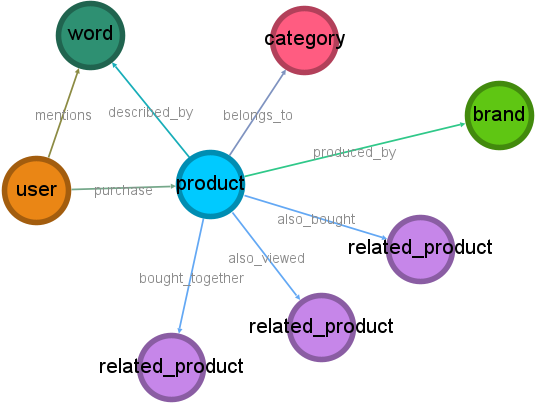
\includegraphics[width=0.6\columnwidth, keepaspectratio]{images/knowledge_graph_structure.png}
		\caption{Structure of the Knowledge Graph}
		\label{fig:knowledge_graph_structure}
	\end{center}
\end{figure}
The enitity types and the relationships between the nodes are demonstrated in
\fref{fig:knowledge_graph_structure}.

\subsection{Path-Based Recommendation Mechanics}
The system operates on predefined metapaths that represent meaningful
relationships leading a user to a product. These metapaths outline the possible structure
of paths that could lead a user to purchase a product.
\begin{figure}[h!]
	\begin{center}
		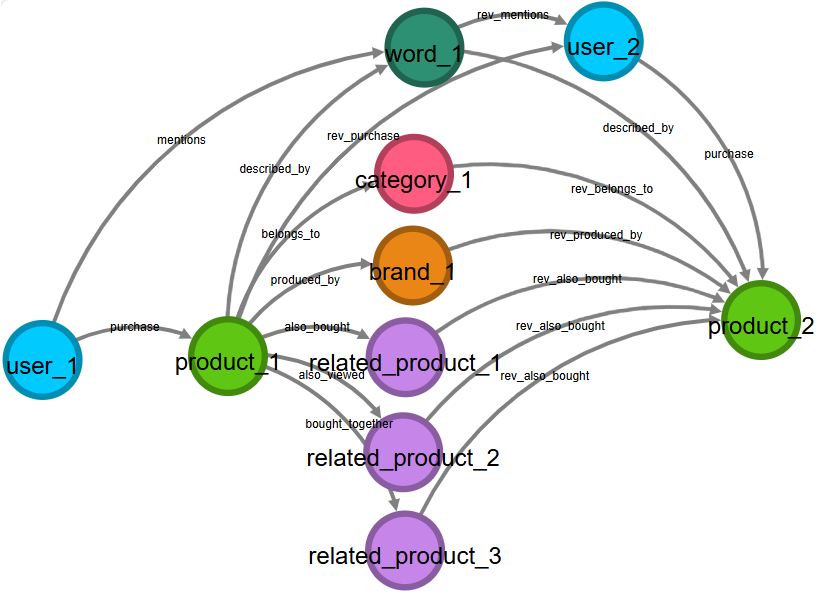
\includegraphics[width=0.9\columnwidth, keepaspectratio]{
			images/metapaths.png
		}
		\caption{Metapaths Definded Within Recommender Systsm}
		\label{fig:metapaths}
	\end{center}
\end{figure}
The structures of metapaths used in the recommeder system at hand are domenstrated
in \fref{fig:metapaths}.

The recommender system assigns a probability score to each step along the path, determining
the strength of the connection between the user and the potential product recommendations.
It then selects the top 10 paths with the highest cumulative scores, and the products
associated with these paths are recommended to the user. This scoring and
selection process ensures that the recommendations are both relevant and
tailored to the user's preferences and behavior patterns. This structured approach
allows the CAFE system to effectively recommend products and offer insights into
the reasons behind each recommendation, enhancing the system's explainability.

\section{Counterfactual Analysis}
\subsection{Outlier Nodes Detection and Removal}

The counterfactual analysis starts by removing outlier nodes from the knowledge
graph. Nodes that exhibit a degree centrality above a certain threshold are eliminated.
While these highly connected nodes can provide valuable insights for
counterfactual analysis, they often include unhelpful elements such as universally
common categories or frequently used words that lack distinctive features.
Additionally, since they disrupt the modularity of communities essential for selecting
relevant attributes, these nodes are removed.

% what is degree centrality
\subsubsection*{Degree Centrality Analysis}
For a given node, degree centrality is the number of edges connected to that node
\parencite{bloch2023centrality}
% how I have calculated the degree centrality for the 


% The graphs of centralities, what that means

% I have experimented with multiple methods, how many nodes are removed, how the modularity changes
% the elbow method

% the qurtile...


\subsection{Community Detection and Graph Analysis Node Filtering}
The next step in the counterfactual analysis is the detection of communities within the knowledge graph of interactions.
Communities are identified using Louvain Method. This helps to cluster entities that
share significant similarities and interactions. The Louvain Method is a an
efficient algorithm designed for detecting communities in large-scale networks
by optimizing modularity, a measure that quantifies the density of links within communities
relative to those between them introduced in \parencite{blondel_fast_2008}. The algorithm operates
in two iterative phases: initially, it optimizes modularity locally, evaluating
potential gains by moving individual nodes into different communities. Nodes are
shifted to the community that maximizes this gain, and the process is repeated
until no further improvement is possible, achieving a local maximum of modularity.
In the second phase, the method aggregates these identified communities into new
nodes of a reduced network, and the process is reapplied. This hierarchical approach
allows the algorithm to uncover community structures at multiple levels effectively.
Notable for its speed, the Louvain Method can handle networks with up to millions
of nodes efficiently, making it well-suited for modern datasets of substantial
size. To refine the analysis further, we calculate the degree centrality for
each type of pair within the graph. Nodes that do not provide significant insight
are filtered out based on their z-score; specifically, nodes with a z-score exceeding
	[specific threshold] are removed.

\subsection{Attribute Selection}
Following the predictions provided by the recommender system, a threshold is set
for the minimum score required for a product path to be recommended to a user, which
is the path score of the last product recommended in the top 10 recommended products.
For the analysis of a recommended path, we retrieve the first-level attributes and
their related products. This forms the initial layer of attribute selection, predicated
on the hypothesis that first-level connected items possess more relevant attributes.
These selected attributes are then evaluated to determine whether they fall
within the community of the recommended product. If they do, and their z-score
is within an acceptable range, they are considered for further counterfactual analysis.

\subsection{Performing Counterfactual Analysis}
For each attribute, an appropriate metapath is selected based on the type of the
attribute. Using the recommender engine, we calculate the score for a user-product
combination, which incorporates all the products previously purchased by the user
and the counterfactual attribute in question. This approach is grounded in the
assumption that the system discerns the user's preferences through their
purchase history. If the recalculated score for a product, when considering a
counterfactual attribute, exceeds the set minimum score, the attribute is
considered a positive influence for a product similar to the recommended one. This
isolated attribute analysis not only aids in understanding the influence of specific
attributes on product recommendations but also provides marketing insights. Such
insights can further be used to enhance the diversity and precision of the
recommender system.

\section{Case Study}